
\chapter{HERO Architecture Simulation}
\label{chap:hero}

so lets say we have a concrete instance of hero-t and we want to assess its
performance in a cycle accurate simulator with real layers from a network. We do
this with a platform simulator that has a front end that takes a mode library
and produces latency, utilization and access cost results.  

\section{Simulation platform}
\label{chap:hero:sim_platform}

Sim runs a CIGAR pass over the input model library if stats dict not available.
It then performs a layer equivelence pass that converts an unsupported
convolution layer to an equivelent GEMM using balanced lowering. Overhead Of
lowering and lifting is automatically added to the overall latency of the cycle
accurate simulation. Simulation only targets conv layers. 

\begin{figure}[ht]
    \centering
    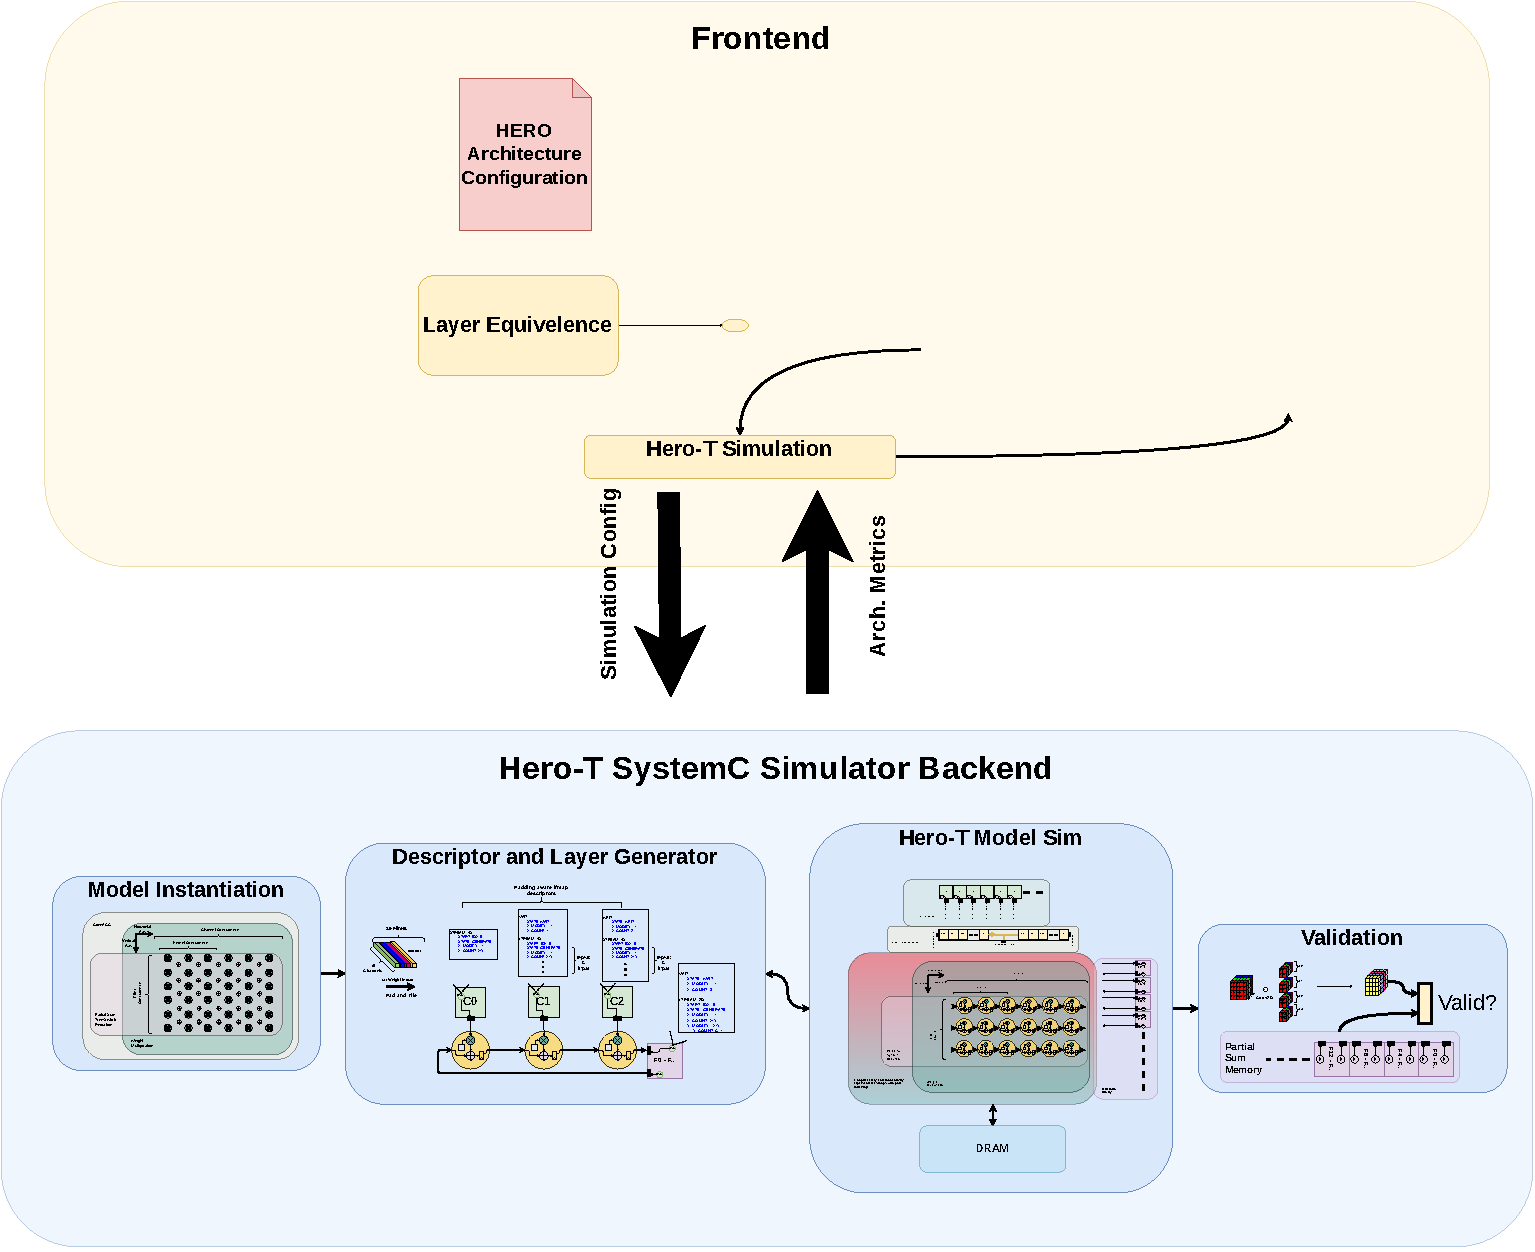
\includegraphics[scale=0.58]{fig/hero-t-sim-platform.pdf}
    \caption{Hardware Implementation Taxonomy adapted from \cite{maestro}}
    \label{fig:hw_taxonomy}
\end{figure}


\section{SystemC Model}
\label{chap:hero:sim_platform:sysc_side}

SystemC models takes in arch config. Arch config usually comes out of a tempo.
Currently systemc model only considers horizontal mapping of kernel loops. All
muxing/ interconnect logic handled with how individual banks are accessed in the
architecture simulation loops. After systemc backend recieves sim config. It
instantiates an arch with the required config. It generates an equivelent layer
following dimensions of layer sent in from front end and then it generates the
descriptor program based on the method discussed in (REFERENCE SAM SUBSECTION)
Finally the backend performs a cycle accurate simulation of the instantiated
architecture. After simulation concludes, ofmap memory contents are scanned to
validate output and if output is valid, latency, access counts and utilization
statistics are returned to the platform frontend for high level analysis. Model
is simulated in isolation. DRAM access counts are estimated in the backend but
no actual simulation of DRAM occurs.

\begin{figure}[ht]
    \centering
    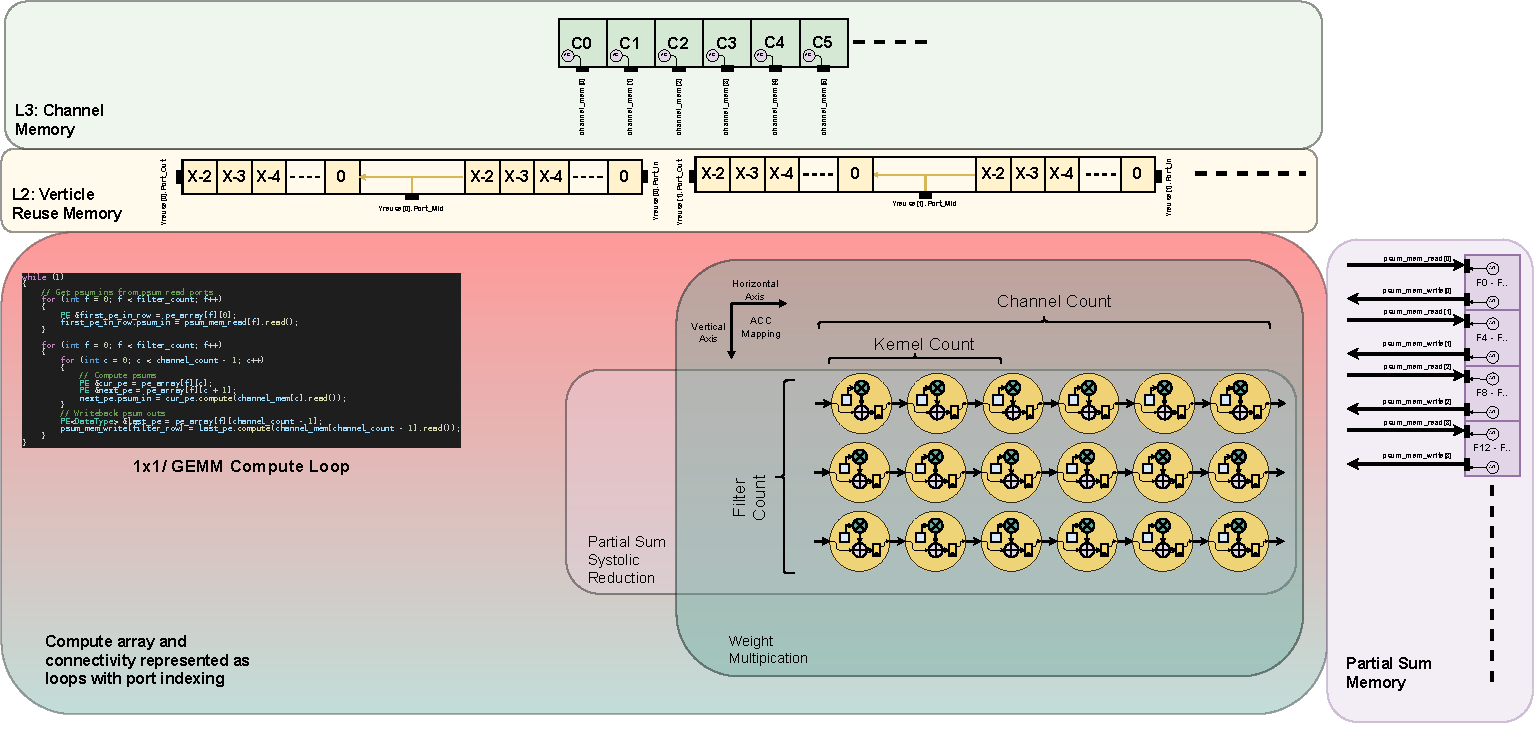
\includegraphics[scale=0.58]{fig/hero-t-sysc.pdf}
    \caption{Hardware Implementation Taxonomy adapted from \cite{maestro}}
    \label{fig:hw_taxonomy}
\end{figure}


\section{Experimental Results}
\label{chap:hero:sim_platform:cigar_side}

Prominent model's convolution layers were are assessed using the simulation platform  
namely resnet-50 mobilenetv3 and vgg16. Performance for each of the three conrete
architectures suggested by tempo is reported below.